\chapter{Introduction}

Write this chapter LAST. Should be 5 to 10 pages. This chapter provides a quick summary of the
essential contents of the research project, principal results and contents of the report. The target
audience is members of the jury who do NOT have time to completely read all 21 reports, as well
academic members of other juries who wish to compare this work to other works.

\section{Background}
This is a generic title. Replace it with an actual title that describes the context of the work.
Short .5 page summary of the technological context of the work and why it is interesting or
important

\section{Problem Statement}
This is a generic title. Replace it with an actual title that describes the context of the work.
Approx .5 to 1 page description of the research problems that was addressed and what was
required to address it.

\section{Scientific Approach and Investigative Method and Results}
This is a generic title. Replace it with an actual title that describes the context of the work.
Approx 1 to 2 page description of the scientific approach or approaches to a solution and how it
was investigated and evaluated. Present a summary of the principal results obtained.

\section{Contents of this report}
Approx .5 page per chapter. Summarize the contents of the subsections of each chapter. Give the
topics addressed and summarize what is written in each chapter. 






\section{Problem Statement}
3D animation can be a painstakingly tedious activity. To create a desired animation, animators go through the long process of keyframing. Keyframes are set positions that define the start and end points of a movement, sequences of poses which are transformed in time. Typically, animators assign poses to certain frames over time, so that in-between motions can be generated by a computer. To get an accurate animation, artists usually must assign many keyframes, then spend time adjusting and editing them to be more precise. The fact that industry professionals take so much time and effort to do this shows that for an amateur or untrained artist, creating \textit{good} 3D animation is close to impossible.

\begin{wrapfigure}{R}{0.6\textwidth}
\centering
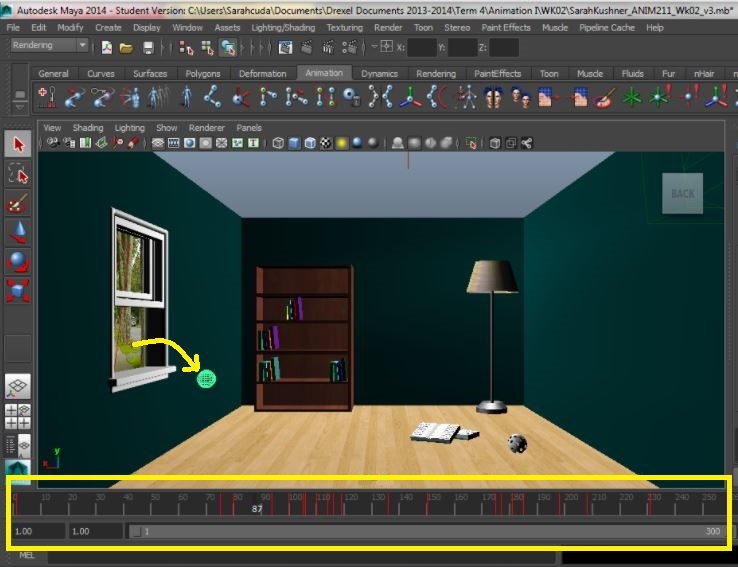
\includegraphics[scale=0.4]{img/keyframe}
\caption{Keyframing.}
\end{wrapfigure}

Researchers in the IMAGINE group at INRIA have noticed this problem. They have made significant progress on a project where they aim to offer more intuitive tools to author 3D digital content. The IMAGINE team has invented (1) a type of notation made especially for posing and animating 3D characters (2) a technique for posing called the line of action, in which a user can draw a line in the shape they want a kinematic chain to take and (3) a technique for animation called space-time sketching, in which a user can draw a line in the path they want a model to take and it will be animated accordingly. As the character follows the path, its model bends and changes shape in a physically realistic way. Their system currently supports creating different movements with the path such as bouncing, rolling, and twisting.

Among the most complicated characters to animate in 3D animation are humanoid characters. To ease this task, animators create a skeleton for their character called a rig, that consists of joints connected by bones to give a structure to the character. Humanoid rigs can range in complexity from (relatively) simple to extremely complicated depending on the amount of detail desired by the user. The structure is a hierarchy of joints that can also be seen as a tree with a root, which in the humanoid case, is usually the pelvis.

\begin{figure}[h!]
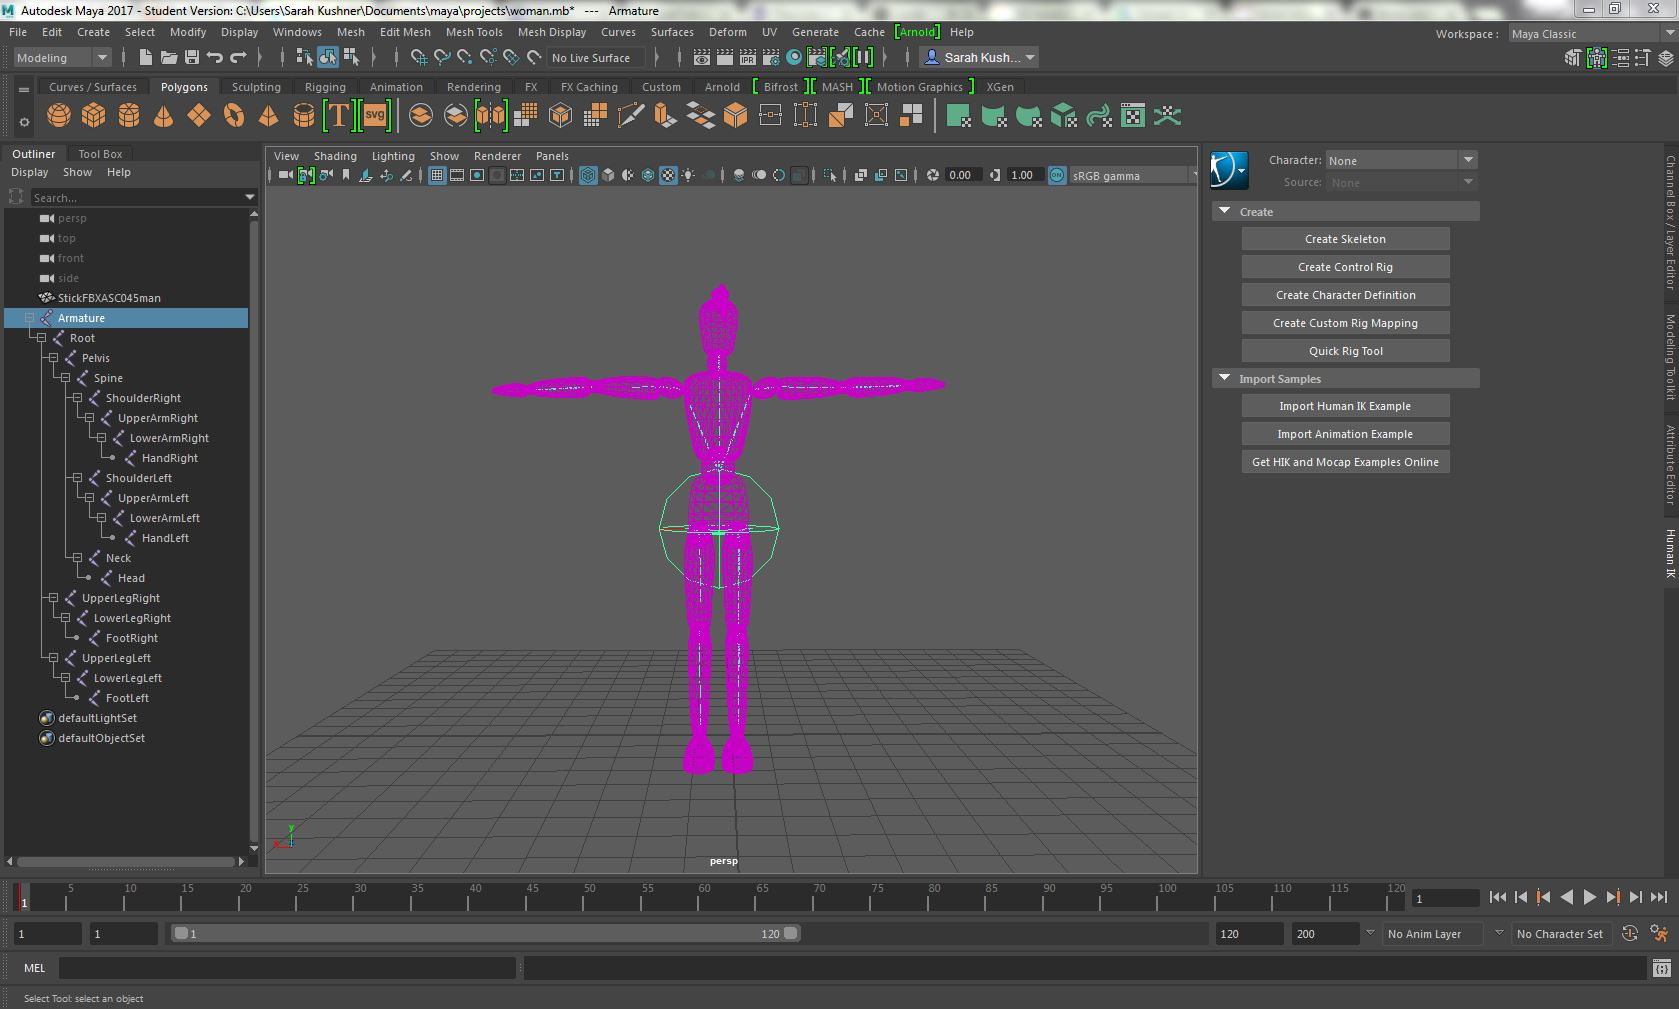
\includegraphics[scale=0.3]{img/skeleton}
\caption{Example of a humanoid skeleton.}
\end{figure}

\section{Forward and Inverse Kinematics}
In order to animate this structure successfully, controls are added that allow for forward and inverse kinematics. These controls help the animator move the character into poses that will then act as keyframes.

Forward kinematics is a method of calculating the position and orientation of the end of a kinematic chain (i.e. a hand or foot) given the positions and angles of the joints higher up in the chain all the way to the root. 

Inverse kinematics is the opposite method of forward kinematics. That is, the goal is to calculate the angles and positions of joints in the chain, given the angle and position of just the end of the chain. This goal much harder to reach, seeing that more information needs to be calculated than is given.

\section{Multiple Characters}
The animation of multiple characters, along with all the previously mentioned challenges, comes with its own unique set as well. The line of action technique works extremely well for a single humanoid character, and even multiple humanoid characters separate from each other. The problem is discovered when the humanoid characters interact, when they are in close proximity to each other or when they touch each other.


Occlusion?

Collisions

\begin{figure}
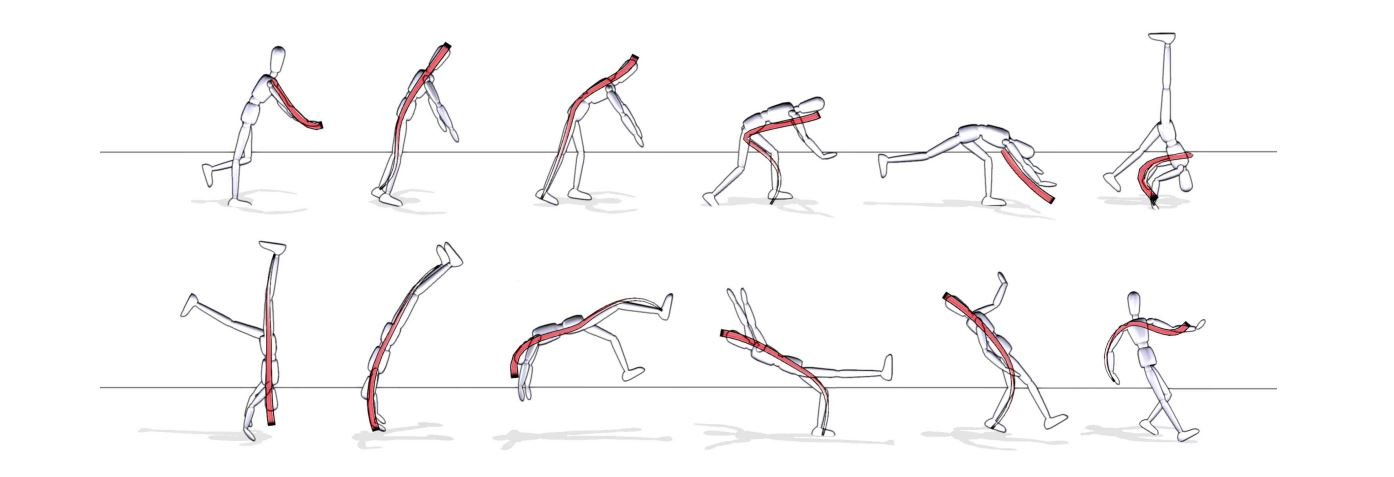
\includegraphics[scale=0.4]{img/baseline}
\caption{One character's keyframes using the line of action technique.}
\end{figure}